\section{递推形式的极限}

有些数列, 常常是利用递推的形式给出的, 如何计算这类数列的极限, 是本节的重点.
此类问题在各类考试中比较常见, 需多加注意.

\subsection{利用存在性求极限}

假若用某种方法证明了递推数列的极限存在, 则在递推公式里取极限, 便可得到极限值 $A$ 应满足的方程, 解此方程, 可求得极限值 $A$.

\begin{theorem}[单调有界准理]
    若 $x_n\nearrow$ 有上界, 或 $x_n\searrow$ 有下界, 则 $\{x_n\}$ 收敛.
    \index{单调有界准理}
\end{theorem}
判断单调性的通常方法有:
\begin{enumerate}[label=(\arabic{*})]
    \item $\displaystyle\forall n\in \mathbb{N}:x_{n+1}-x_n\begin{cases}\geqslant 0,&x_n\nearrow,\\ \leqslant 0,&x_n\searrow.\end{cases}$
    \item $\displaystyle\forall n\in\mathbb{N}:\frac{x_{n+1}}{x_n}\begin{cases}\geqslant 1,&x_n\nearrow,\\ \leqslant 1,&x_n\searrow.\end{cases}$
    \item 若 $x_{n+1}=f(x_n),~f'(x)\geqslant 0\text{, 则 }\begin{cases}x_1\leqslant x_2,&x_n\nearrow,\\ x_1\geqslant x_2,&x_n\searrow.\end{cases} $
\end{enumerate}

\begin{theorem}[压缩映射]
    对于任一数列 $\{x_n\}$ 而言, 若存在常数 $r$, 使得 $\forall n\in\mathbb{N}$, 恒有
    $$|x_{n+1}-x_n |\leqslant r|x_n-x_{n-1} |,~0<r<1$$
    则数列 $\{x_n\}$ 收敛;特别地, 若数列 $\{x_n\}$ 利用递推公式给出: $x_{n+1}=f(x_n)~  (n=1,2,\cdots)$, 
    其中 $f$ 为某一可微函数, 且 $\exists r\in \mathbb{R}$, 使得
    $$|f'(x)|\leqslant r<1$$
    则数列 $\{x_n\}$ 收敛. 若上式只在某区间 $D$ 上成立, 则必须验证数列 $\{x_n\}$ 是否保持在区间 $D$ 内.
    \index{压缩映射}
\end{theorem}
\begin{theorem}[不动点迭代]
    求解非线性方程 (组) 的一类常见的数值解法. 例如, 单个方程的求根问题 $f(x)=0$ 总可以等价地写成 $x=\phi (x)$, 
    其中 $\phi:\mathbb{R}\to\mathbb{R}$ 是一个辅助函数, 满足该式的点 $x$ 称为不动点.
    如果给定初始点 $x{(0)}$, 就可以考虑如下的不动点迭代法: $$x^{(k+1)}=\phi\left(x^{(k)}\right)~  (k=0,1,\cdots)$$
    函数 $\phi$ 亦称为\textbf{迭代函数}.

    如果迭代函数 $\phi$ 是一个闭区间上的压缩映射 (或者迭代函数连续可微, 且导数的绝对值在该闭区间上严格小于 $1$), 
    则不动点迭代法产生的序列 $\{x^{(k)}\}$ 收敛到 $\phi$ 在区间上的不动点.
    \index{不动点迭代}
\end{theorem}
\begin{figure}[H]
    \centering
    \begin{tikzpicture}[samples=100,>=stealth,domain=0:4]
        \coordinate (xMin) at (-0.5,0);
        \coordinate (xMax) at (5,0);
        \coordinate (yMin) at (0,-0.5);
        \coordinate (yMax) at (0,4.5);
        \draw[->,cyan] (xMin)--(0,0) node [below left] {$O$}--(xMax) node[below] {$x$};
        \draw[->,cyan] (yMin)--(yMax) node [left] {$y$};
        \path[draw,name path=x,semithick] plot(\x,\x) node[right] {$y=x$};
        \path[draw,name path=f(x),semithick,domain=0.3:4] plot(\x,{0.5*(\x+2/(\x))}) node[right] {$f(x)=x$};
        \path[name intersections={of=x and f(x),by=A}];
        \node[below,magenta] at (A) {$A^*$};
        \draw[densely dashed,magenta] node[below] at (0.35,0) {$A_1$}
        (0.35,0)--(0.35,{0.5*(0.35+2/0.35)}) node[above right] {$A_2$}
        --({0.5*(0.35+2/0.35)},{0.5*(0.35+2/0.35)}) node[above left] {$A_2'$}
        --({0.5*(0.35+2/0.35)},{0.5*((0.5*(0.35+2/0.35))+2/(0.5*(0.35+2/0.35)))}) node[below] {$A_3$}
        --({0.5*((0.5*(0.35+2/0.35))+2/(0.5*(0.35+2/0.35)))},{0.5*((0.5*(0.35+2/0.35))+2/(0.5*(0.35+2/0.35)))}) node[above left] {$A_3'$}
        --({0.5*((0.5*(0.35+2/0.35))+2/(0.5*(0.35+2/0.35)))},{0.5*((0.5*((0.5*(0.35+2/0.35))+2/(0.5*(0.35+2/0.35))))+2/(0.5*((0.5*(0.35+2/0.35))+2/(0.5*(0.35+2/0.35)))))}) node[below] {$A_4$}
        --({0.5*((0.5*((0.5*(0.35+2/0.35))+2/(0.5*(0.35+2/0.35))))+2/(0.5*((0.5*(0.35+2/0.35))+2/(0.5*(0.35+2/0.35)))))},{0.5*((0.5*((0.5*(0.35+2/0.35))+2/(0.5*(0.35+2/0.35))))+2/(0.5*((0.5*(0.35+2/0.35))+2/(0.5*(0.35+2/0.35)))))}) node[above left] {$A_4'$};
    \end{tikzpicture}
    \caption{}
\end{figure}
\begin{example}
    设数列 $\{x_n\}$ 满足: $x_0=1,~x_{n+1}=\sqrt{2x_n}~  (n=0,1,2,\cdots)$, 证明 $\{x_n\}$ 收敛, 并求极限值.
\end{example}
\begin{proof}[{\songti \textbf{证法一}}]
    $\displaystyle x_{n}=\sqrt{2x_{n-1}}=\sqrt{2\sqrt{2x_{n-2}}}=\sqrt{2\sqrt{2\sqrt{\cdots\sqrt{2}}}}=2^{\frac{1}{2}+\frac{1}{2^{2}}+\cdots +\frac{1}{2^{n}}}=2^{1-\frac{1}{2^{n}}}\to2~  (n\to\infty).$
\end{proof}
\begin{proof}[{\songti \textbf{证法二}}]
    显然 $1\leqslant x_0<2$, 假设 $1\leqslant x_k<2$, 则 $1\leqslant x_{k+1}=\sqrt{2x_k}<\sqrt{2\cdot 2}=2$, 故由数学归纳法知, $\forall n\in\mathbb{N}:1\leqslant x_n<2$, 
    又由 $\dfrac{x_{n+1}}{x_n}=\dfrac{\sqrt{2x_n}}{x_n}=\sqrt{\dfrac{2}{x}}>1$, 知 $\{x_n\}\nearrow$, 所以由单调有界原理得 $\{x_n\}$ 收敛, 不妨记 $\lim\limits_{n\to\infty}x_n=A$, 则在递推公式里取极限, 
    有 $A=\sqrt{2A}\Rightarrow A=0,2$, 而由 $x_n\ge1$, 知 $A\geqslant 1$, 故取 $A=2$, 即 $\lim\limits_{n\to\infty}x_n=A.$
\end{proof}
\begin{proof}[{\songti \textbf{证法三}}]
    令 $f(x)=\sqrt{2x}~  (x>0)$, 则 $f'(x)=\dfrac{1}{\sqrt{2x}}>0~  (x>0)$, 于是当 $x>0$ 时, $f(x)\nearrow$, 从而有 $x_n>x_{n-1}$, 可得
    $x_{n+1}=f(x_n)>f(x_{n-1})=x_n$, 而 $x_1=\sqrt{2}>x_0=1$, 故有 $x_1<x_2<\cdots$, 即 $\{x_n\}\nearrow$, 其余证法同证法 2.
\end{proof}
\begin{proof}[{\songti \textbf{证法四}}]
    如证法 2, 已有 $1\leqslant x_n <2$, 对 $f(x)=\sqrt{2x}$, 有$$|f'(x)|=\dfrac{\sqrt{2}}{2\sqrt{x}}\leqslant\dfrac{\sqrt{2}}{2}<1$$
    满足压缩映射条件, 其余证法同证法 2.
\end{proof}
\begin{proof}[{\songti \textbf{证法五}}]
    由递推关系式两边取对数, 得 $\ln x_{n+1}=\dfrac{1}{2}\ln x_n+\dfrac{1}{2}\ln 2$, 令 $b_n=\ln x_n$, 则
    $$b_{n+1}=\dfrac{1}{2}b_{n}+\dfrac{1}{2}\ln 2,~b_0=0$$
    记 $f(x)=\dfrac{1}{2}x+\dfrac{1}{2}\ln 2$, 则 $b_{n+1}=f(b_n)$, 又由特征方程 $x=f(x)$, 解得特征根 $x=\ln 2$, 所以
    \begin{flalign*}
        b_n-\ln 2 =\left(\dfrac{1}{2}b_{n-1}+\dfrac{1}{2}\ln 2\right)-\left(\dfrac{1}{2}\ln 2+\dfrac{1}{2}\ln 2\right)=\dfrac{1}{2}(b_{n-1}-\ln 2)
        =\left(\dfrac{1}{2}\right)^n\cdot(b_0-\ln 2)=-\ln 2\cdot\left(\dfrac{1}{2}\right)^n
    \end{flalign*}
    于是 $\lim\limits_{n\to\infty}(b_n-\ln 2)=0$, 即 $\lim\limits_{n\to\infty}x_n=2.$
\end{proof}
\begin{inference}
    一般地, 设 $a,x_0>0,x_{n+1}=\sqrt{ax}~  (n=0,1,2,\cdots)$, 则数列 $\{x_n\}$ 收敛, 且 $\lim\limits_{n\to\infty}x_n=a.$
\end{inference}

\begin{example}
    已知 $x_1=\sqrt{6},~x_n=\sqrt{6+x_{n-1}}~  (n=2,3,\cdots)$, 证明数列 $\{x_n\}$ 有极限, 并求其值.
\end{example}
\begin{proof}[{\songti \textbf{证法一}}]
    用数学归纳法可证: $0<x_n<3~  (n=1,2,\cdots)$, \\
    因为 $x_{n+1}x-{n}=\sqrt{6+x_n}-\sqrt{6+x_{n-1}}=\dfrac{x_n-x_{n-1}}{\sqrt{6+x_n}+\sqrt{6+x_{n-1}}}$, 所以 $x_{n+1}-x_n$ 与 $x_n-x_{n-1}$ 同号, 
    又 $x_2=\sqrt{6+\sqrt{6}}>\sqrt{6}=x_1$, 所以 $x_{n+1}>x_{n}$, 即 $\{x_n\}\nearrow 3$, 由单调有界准则知, $\{x_n\}$ 收敛.
\end{proof}
\begin{proof}[{\songti \textbf{证法二}}]
    先假设数列 $\{x_n\}$ 收敛, 不妨设 $\lim\limits_{n\to\infty}x_n=A$, 则由递推关系式两边取极限, 得 $A=\sqrt{6+A}$, 解得 $A=3,-2$, 
    因为 $x_n>0~  (n=1,2,\cdots)$, 所以 $A=3$, 下证数列 $\{x_n\}$ 收敛于 $3$.\\
    记 $q=\dfrac{1}{\sqrt{6}+3}$, 则有
    $$|x_n-3|=\left|\sqrt{6+x_{n-1}}-3\right|=\dfrac{|x_{n-1}-3|}{\sqrt{6+x_{n-1}}+3}<q\cdot|x_{n-1}-3|<\cdots<q^{n-1}\cdot|x_1-3|$$
    而由 $\lim\limits_{n\to\infty}q^n=0$, 故由极限的定义或者夹逼准则, 可得 $\lim\limits_{n\to\infty}x_n=3.$
\end{proof}

\begin{example}
    已知数列 $ \left\{x_{n}\right\} $ 满足 $ x_{n+1}=\dfrac{x_{n}^{2}}{2\left(x_{n}-1\right)},(n=0,1,2, \cdots)  $, 且 $ x_{0}>1$, 证明: 数列 $ \left\{x_{n}\right\} $ 收敛, 并求其极限.
\end{example}
\begin{solution}
    因为 $x_{n+1}=\dfrac{x_n^2}{2(x_n-1)}=\dfrac{x_n^2-1+1}{2(x_n-1)}=\dfrac{(x_n-1)(x_n+1)+1}{2(x_n-1)}=1+\dfrac{x_n-1}{2}+\dfrac{1}{2(x_n-1)}\geqslant 2~~(n=1,2,\cdots)$, \\
    \begin{minipage}{0.29\linewidth}
        \begin{figure}[H]
            \centering
            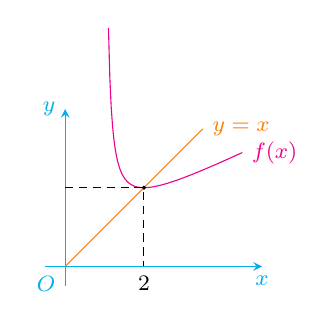
\begin{tikzpicture}[->,samples=100,>=stealth,font=\footnotesize,scale=0.5]
                \draw[->,cyan](-0.5,0)--(0,0)node[below left]{$O$}--(5,0)node[below]{$x$};
                \draw[->,cyan](0,-0.5)--(0,4)node[left]{$y$};
                \draw[-,magenta,domain=1.1:4.5]plot(\x,{\x*\x/(2*\x-2)})node[right]{$f(x)$};
                \draw[orange,-,domain=0:3.5]plot(\x,{\x})node[right]{$y=x$};
                \draw[densely dashed,-](0,2)--(2,2)--(2,0)node[below]{$2$};
                \draw[fill=black] (2,2) circle(1pt);
            \end{tikzpicture}
            \caption{}
            \label{bddxn2xn1}
        \end{figure}
    \end{minipage}\hfill
    \begin{minipage}{0.7\linewidth}
        \textbf{法一: }令 $f(x)=\dfrac{x^2}{2(x-1)}$, 则
        $$f'(x)=\dfrac{x(x-2)}{2(x-1)^2}=\dfrac{1}{2}\qty[1-\dfrac{1}{(x-1)^2}]$$
        所以 $|f'(x)|=\qty|\dfrac{1}{2}\qty[1-\dfrac{1}{(x-1)^2}]|<\dfrac{1}{2}<1$, 表明 $x_{n+1}=f(x_n)$ 是一压缩映像, 所以 $\qty{x_n}$ 收敛, 即 $\displaystyle\lim_{n\to\infty}x_n$ 存在, 不妨记为 $A$, 对 $x_{n+1}=\dfrac{x_n^2}{2(x_n-1)} $ 两边取极限, 有
        $A=\dfrac{A^2}{2(A-1)}\Rightarrow A=2$, 由极限的保序性可得 $A=2$, 即原数列极限为 2.\\
        \textbf{法二: }$x_{n+1}-x_n=\dfrac{x_n^2}{2(x_n-1)}-x_n=-\dfrac{x_n(x_n-2)}{2(x_n-1)}<0$, 则 $\qty{x_n}\searrow$, 同法一可得数列极限为 2.
    \end{minipage}
    \textbf{法三: }取\footnote{由图 \ref{bddxn2xn1} 可知在 $x>1$ 处有一个不动点 $x=2$.} $A=2$, 则 $A=\dfrac{A^2}{2(A-1)}$, 作 
    \begin{flalign*}
        \qty|x_{n+1}-A|-\qty|\dfrac{x_n^2}{2(x_n-1)}-\dfrac{A^2}{2(A-1)}|&=\dfrac{1}{2}\qty|\dfrac{x_n^2-1+1}{x_n-1}-\dfrac{A^2-1+1}{A-1}|=\dfrac{1}{2}\qty|x_n+1+\dfrac{1}{x_n-1}-(A+1)-\dfrac{1}{A-1}|\\
        &=\dfrac{1}{2}\qty|x_n-A+\dfrac{1}{x_n-1}-\dfrac{1}{A-1}|<|x_n-A|
    \end{flalign*}
    因此 $$\qty|x_{n+1}-A|<\dfrac{1}{2}\qty|x_n-A|<\cdots<\dfrac{1}{2^{n+1}}\qty|x_0-A|\to 0~~(n\to\infty)$$
    故由夹逼准则 (或数列极限的定义) 可知 $\displaystyle\lim_{n\to\infty}x_n=2.$
\end{solution}

\begin{example}
    (试用三种方法求) 设 $x_1>0,~x_{n+1}=\dfrac{c(1+x_n)}{c+x_n}~  (c \text{为常数})$, 求 $\lim\limits_{n\to\infty}x_n.$
\end{example}
\begin{solution}
    \textbf{法一: }(用单调有界准则) 若 $x_1=\sqrt{c}$, 则 $x_n=\sqrt{c}~  (\forall n\in\mathbb{N}),~\lim\limits_{n\to\infty}x_n=\sqrt{c}$, 
    若 $x_1>\sqrt{c}$, 因 $f(x):=\dfrac{c(1+x_n)}{c+x}=c-\dfrac{c(c-1)}{c+x}$ 严格 $\nearrow$, 故 $\forall n\in\mathbb{N}:x_n>\sqrt{c}\Rightarrow x_{n+1}=\dfrac{c(1+x_n)}{c+x_n}=f(x_n)>f\left(\sqrt{c}\right)=\sqrt{c}$, 
    由 $x_1>\sqrt{c}$ 可递推出 $x_n\sqrt{c}$, 又因为 $x_{n+1}-x_{n}=\dfrac{c-x_n^2}{c+x_n}<0$, 知 $x_n$ 严格 $\nearrow$, 故 $\{x_n\}$ 收敛, 
    同理可证, 当 $0<x_1<\sqrt{c}$ 时, $x_n\nearrow\sqrt{c}$, 综上, $\{x_n\}$ 单调有界, 极限存在, 令递推式 $\dfrac{c(1+x_n)}{c+x_n}$ 两边取极限, 得极限为 $\sqrt{c}.$\\
    \textbf{法二: }(用压缩映射) 因为 $x_n>0$, 且 $x>0$ 时, $f'(x)=\left[\dfrac{c(1+x)}{c+x}\right]'=\dfrac{c(c-1)}{(c+x)^2}>0$, 又 $c>1$ 知
    $$0<f'(x)=\dfrac{c(c-1)}{(c+x)^2}\leqslant\dfrac{c(c-1)}{c^2}=1-\dfrac{1}{c}<1~  (\forall x>0)$$
    故 $x_{n+1}=f(x_n)$ 为压缩映射, $\{x_n\}$ 收敛, 同上由 $\lim\limits_{n\to\infty}x_n=\sqrt{c}.$\\
    \textbf{法三: }显然对一切 $x_n>0$, 令 $f(x)=\dfrac{c(1+x)}{c+x}=x$, 知不动点 $x^*=\sqrt{c}$, 而 $f\nearrow$ 保证了 $x_n$ 位于不动点 $x^*$ 的同一侧, 且
    $$\left[x-\dfrac{c(1+x)}{c+x}\right]\left(x-\sqrt{c}\right)=\dfrac{cx+x^2-c-cx}{c+x}\left(x-\sqrt{c}\right)=\dfrac{x+\sqrt{c}}{c+x}\left(x+\sqrt{c}\right)^2>0$$
    意味着 $x_n$ 向 $x^*$ 步步靠近, 根据不动点迭代法知, $\lim\limits_{n\to\infty}x_n=\sqrt{c}.$
\end{solution}

\begin{example}
    设 $a,x_0>0,~x_{n+1}=\dfrac{1}{2}\left(x_n+\dfrac{a}{x_n}\right)~  (n=0,1,\cdots)$, 证明数列 $\{x_n\}$ 收敛, 并求其值.
\end{example}
\begin{proof}[{\songti \textbf{证法一}}]
    由算术平均数大于几何平均数得 $x_{n+1}=\dfrac{1}{2}\left( x_{n}+\dfrac{a}{x_{n}}\right) \geqslant \sqrt{a}~  (n= 0,1,2,\cdots) $, 于是
    $\dfrac{x_{n+1}}{x_{n}}=\dfrac{1}{2}\left( 1+\dfrac{a}{x_{n}^{2}}\right) \leqslant 1$, 即 $x_{n+1}\leqslant x_{n}$, 从而数列 $\{x_n\}\searrow\sqrt{a}$, 故数列收敛, 
    设 $\lim\limits_{n\to\infty}x_n=A$, 则由递推关系式两边取极限解得 $A=\pm\sqrt{a}$, 因为 $x_n\geqslant \sqrt{a}$, 所以极限为 $\sqrt{a}.$
\end{proof}
\begin{proof}[{\songti \textbf{证法二}}]
    由已知 $x_n>0$, 且
    \begin{flalign*}
        x_{n+1}-x_{n} & =\dfrac{1}{2}\left( x_{n}+\dfrac{a}{x_{n}}\right) -x_{n}=\dfrac{1}{2}\left( \dfrac{a}{x_{n}}-x_{n}\right) =\dfrac{1}{2}\left[ \dfrac{a}{\dfrac{1}{2}\left( x_{n-1}+\dfrac{a}{x_{n-1}}\right) }-\dfrac{1}{2}\left( x_{n-1}+\dfrac{a}{x_{n-1}}\right) \right] \\
                      & =\dfrac{1}{4}\cdot\dfrac{-\left(x_{n-1}^2-a\right)^a}{x_{n-1}\cdot\left(x_{n-1}^2+a\right)}<0~  (n\geqslant 2)
    \end{flalign*}
    所以 $\{x_n\}\searrow 0$, 同解法 1, 可求得极限值为 $\sqrt{a}$.
\end{proof}
\begin{proof}[{\songti \textbf{证法三}}]
    由 $x_{n+1}=\dfrac{1}{2}\left(x_n+\dfrac{a}{x_n}\right)\geqslant \sqrt{a}~  (n=0,1,2,\cdots)$, 所以 $x_{n+1}-\sqrt{a}=\left(x_n-\sqrt{a}\right)\cdot\dfrac{1}{2}\left(1-\dfrac{\sqrt{a}}{x_n}\right)$, 
    反复利用该递推公式, 得
    $$x_{n+1}-\sqrt{a}=\left( x_{1}-\sqrt{a}\right) \cdot \dfrac{1}{2^{n}}\left( 1-\dfrac{\sqrt{a}}{x_{1}}\right) \left( 1-\dfrac{\sqrt{a}}{x_{2}}\right) \cdots \left( 1-\dfrac{\sqrt{a}}{x_{n}}\right) $$
    于是 $\left|x_{n+1}-\sqrt{a}\right|\leqslant\dfrac{1}{2^n}\cdot\left|x_{1}-\sqrt{a}\right|$, 因为 $\lim\limits_{n\to\infty}\dfrac{1}{2^n}=0$, 由夹逼准则得 $\left|\lim\limits_{n\to\infty}x_{n+1}-\sqrt{a}\right|=0$, 
    故 $\lim\limits_{n\to\infty}x_n=\sqrt{a}.$
\end{proof}
\begin{inference}
    一般地, 设 $a,x_1>0,m\in\mathbf{N^*},~x_{n+1}=\dfrac{1}{m}\left[ \left( m-1\right) x_{n}+\dfrac{a}{x_{n}^{m-1}}\right] $, 则 $\lim\limits_{n\to\infty}x_n=\sqrt[m]{a}.$
\end{inference}
\begin{example}
    设 $a,x_0>0,x_{n+1}=\dfrac{x_n\left(x_n^2+3a\right)}{3x_n^2+a}~  (n=0,1,\cdots)$, 证明数列 $\{x_n\}$ 收敛, 并求极限值.
\end{example}
\begin{proof}
    令 $f(x)=\dfrac{x(x^2+3a)}{3x^2+a}$, 则 $f'(x) =\dfrac{3\left( x^{2}-a^{2}\right) ^{2}}{\left( 3x^{2}+a\right) ^{2}}\geqslant 0,x_{n+1}=f(x_n)$, \\
    若 $x_0\geqslant \sqrt{a}$, 则 $x_1=f(x_0)\geqslant f\left(\sqrt a\right)=\sqrt{a}$, 由 $x_n\geqslant \sqrt{a}$ 可得 $x_{n+1}=f(x_n)\geqslant f\left(\sqrt{a}\right)=\sqrt{a}$, 
    于是由数学归纳法得 $\forall n\in\mathbb{N},x_n\geqslant\sqrt{a}$, 又 $x_1=\dfrac{x_0\left(x_0^2+3a\right)}{3x_0^2+a}\leqslant x_0$, 由 $f'(x)\geqslant 0$ 得 $x_2=f(x_1)\leqslant f(x_0)=x_1$, 反复利用此关系, 
    即得 $x_{n+1}\leqslant x_n$, 于是数列 $\{x_n\}\searrow\sqrt{a}$, 故数列 $\{x_n\}$ 收敛, \\
    若 $0<x_0<\sqrt{a}$, 则类似上面可证得 $\forall n\in\mathbb{N},0<x_n<\sqrt{a}$ 且 $x_{n+1}\geqslant x_{n}$, 于是数列 $\{x_n\}\nearrow\sqrt{a}$, 故数列 $\{x_n\}$ 收敛, 
    不妨设 $\lim\limits_{n\to\infty}x_n=A$, 易得 $\lim\limits_{n\to\infty}x_n=\sqrt{a}.$
\end{proof}
\begin{inference}
    一般地, 设 $k\geqslant 2,k\in\mathbb{N}^*,x_0>0$, 令 $x_{n+1}=\dfrac{\displaystyle x_{n}^{k}+\sum\limits ^{\left[ k/2\right] }_{i=1}\mathrm{C}_{k}^{2i}\cdot x_{n}^{k-2i}\cdot a^{i}}{\displaystyle\sum\limits ^{\left[ \left( k-1\right) /2\right] }_{i=0}\mathrm{C}_{k}^{2i+1}\cdot x_{n}^{k-2i-1}\cdot a^{i}}~  (n=0,1,\cdots)$, 
    则数列 $\{x_n\}$ $k$ 阶收敛于 $\sqrt{a}.$

    事实上, 因为 $\dfrac{x_{n+1}-\sqrt{a}}{x_{n+1}+\sqrt{a}}=\left( \dfrac{x_{n}-\sqrt{a}}{x_{n}+\sqrt{a}}\right) ^{k}=\cdots =\left( \dfrac{x_{1}-\sqrt{a}}{x_{1}+\sqrt{a}}\right) ^{k^{n}}$, 
    所以有 $$x_{n+1}-\sqrt{a}=2\sqrt{a}\dfrac{\gamma ^{k^{n}}}{1-\gamma ^{k^{n}}}\rightarrow 0\left( n\rightarrow \infty \right) $$
    且有
    $$\lim _{n\rightarrow \infty }\dfrac{x_{n+1}-\sqrt{a}}{\left( x_{n}-\sqrt{a}\right) ^{k}}=\lim _{n\rightarrow \infty }\dfrac{x_{n+1}+\sqrt{a}}{\left( x_{n}+\sqrt{a}\right) ^{k}}=\dfrac{1}{\left( 2\sqrt{a}\right) ^{k-1}}.$$
\end{inference}

\subsection{写出通项求极限}

\subsubsection{利用不动点求通项}

在前小节介绍了不动点迭代法, 下文将介绍如何运用不动点解决两种类型的数列通项问题.

\begin{example}
    已知 $a_{n+1}=\dfrac{a\cdot a_n+b}{c\cdot a_n+d}~  (c\not=0)$, 且 $ad-bc\not=0$, $a,b,c,d$ 都是常数, 求通项 $a_n$.
\end{example}
\begin{solution}
    设 $f(x)=\dfrac{ax+b}{cx+d}~  (c,ad-bc\not=0)$, $\{a_n\}$ 满足递归关系 $a_{n+1}=f(a_n)$, 且初始值 $a_1\not=f(a_1)$.
    \begin{enumerate}[label=(\arabic{*})]
        \item 若 $f$ 有两相异的不动点 $p,q$, 则 $\dfrac{a_{n+1}-p}{a_{n+1}-q}=k\cdot \dfrac{a_{n}-p}{a_{n}-q}$, 其中 $k=\dfrac{a-pc}{b-qc}$, 即
              $\left\{\dfrac{a_n-p}{a_n-q}\right\}$ 是以 $k$ 为公比的等比数列, 由此解得
              $$a_{n}=\dfrac{\left( a_1q-pq\right) k^{n-1}-\left( a_1p-pq\right) }{\left( a_1-p\right) k^{n-1}-\left( a_1-q\right) }.$$
        \item 若 $f$ 只有一个不动点 $p$, 则 $\dfrac{1}{a_{n+1}-p}=\dfrac{1}{a_{n}-p}+k$, 其中 $k=\dfrac{2c}{a+d}$, 
              即 $\left\{\dfrac{1}{a_n-p}\right\}$ 是以 $k$ 为公差的等差数列, 由此解得
              $$a_{n}=\dfrac{a_{1}-p}{\left( ka_{1}-pk\right) n+1-ka_{1}+pk}+k.$$
    \end{enumerate}
\end{solution}
\begin{example}
    已知 $a_{n+1}=\dfrac{a\cdot a_n^2+b}{2a \cdot a_n+c}~  (a\not=0)$, $a,b,c$ 都是常数, 求通项 $a_n$.
\end{example}
\begin{solution}
    设递归函数为 $f(x)=\dfrac{ax^2+b}{2ax+c}$, 那么
    \begin{enumerate}
        \item 若 $f$ 有两相异的不动点 $p,q$, 即 $p=\dfrac{ap^2+b}{2ap+c},~q=\dfrac{aq^2+b}{2aq+c}$, 则
              $$a_{n+1}-p=\dfrac{a\cdot an^{2}+b}{2a\cdot a_{n}+c}-p=\dfrac{a\cdot a_{n}^{2}+b-2apa_{n}-pc}{2a\cdot a_{n}+c}=\dfrac{a\cdot a_{n}^{2}-2apa_{n}+ap^{2}}{2a\cdot a_{n}+c}=\dfrac{a(a-p)^2}{2a\cdot a_n+c}$$
              同理 $a_{n+1}-q=\dfrac{a\left( a_{n}-q\right) ^{2}}{2a\cdot a_{n}+c}$, 两式相除, 得
              $$\dfrac{a_{n+1}-p}{a_{n+1}-q}=\left(\dfrac{a_n-p}{a_n-q}\right)^2=\left(\dfrac{a_{n-1}-p}{a_{n-1}-q}\right)^{2^2}=\cdots=\left(\dfrac{a_1-p}{a_1-q}\right)^{2^{n-1}}$$
              由此解得, $a_{n}=\dfrac{q\left( a_{1}-p\right) ^{2^{n-1}}-p\left( a_1-q\right)^ {2^{n-1}}}{\left( a_{1}-p\right) ^{2^{n-1}}-\left( a_{1}-q\right) ^{2^{n-1}}}.$
        \item 若 $f$ 有两相同的不动点 $p$, 易得 $p=-\dfrac{c}{2a}$, 由 $a_{n+1}-p=a_{n+1}+\dfrac{c}{2a}=\dfrac{a\cdot a_n^2+b}{2a\cdot a_n+c}+\dfrac{c}{2a}$, 令 $b_n=a_n+\dfrac{c}{2a_n}$, 化简可得 $b_{n+1}=\dfrac{1}{2}b_n$, 
              即 $b_n=\left(a_1+\dfrac{c}{2a}\right)\left(\dfrac{1}{2}\right)^{n-1}$, 由此解得
              $$a_{n}=\left( a_{1}+\dfrac{c}{2a}\right) \left( \dfrac{1}{2}\right) ^{n-1}-\dfrac{c}{2a}.$$
    \end{enumerate}
\end{solution}
\begin{example}
    设数列 $\{x_n\}$ 满足 $x_1=2,x_{n+1}=2+\dfrac{1}{x_n}~  (n=1,2,\cdots)$, 证明数列 $\{x_n\}$ 收敛, 并求 $\lim\limits_{n\to\infty}x_n.$
\end{example}
\begin{proof}[{\songti \textbf{证法一}}]
    记 $f(x)=2+\dfrac{1}{x}$, 则 $x_{n+1}=f(x_n)$, 由 $f(x)=x$ 解得不动点为 $p=1+\sqrt{2},q=1-\sqrt{2}$, 于是
    $$\dfrac{x_{n}-p}{x_{n}-q}=\dfrac{q}{p}\cdot \dfrac{x_{n-1}-p}{x_{n-1}-q}=\cdots=\left( \dfrac{q}{p}\right) ^{n-1}\cdot \dfrac{x_{1}-p}{x_{2}-q}$$
    而 $\left| \dfrac{q}{p}\right| =\left| \dfrac{1-\sqrt{2}}{1+\sqrt{2}}\right|  <1$, 故 $\lim\limits_{n\to\infty}\dfrac{x_n-p}{x_n-q}=0\Rightarrow \lim\limits_{n\to\infty}x_n=1+\sqrt{2}.$
\end{proof}
\begin{proof}[{\songti \textbf{证法二}}]
    假设数列 $\{x_n\}$ 的极限存在, 不妨设 $\lim\limits_{n\to\infty}x_n=a$, 则由递推关系式两边取极限解得 $a=1\pm\sqrt{2}$, 又因为 $$x_{n+1}=\dfrac{1}{x_n}+2>2$$
    所以 $a\geqslant 2$, 故取 $a=1+\sqrt{2}$, 下证数列 $\{x_n\}$ 的极限存在, 
    \begin{flalign*}
        \left| x_{n}-a\right| & =\left| \left( 2+\dfrac{1}{x_{n}-1}\right) -\left( 2+\dfrac{1}{a}\right) \right| =\left| \dfrac{1}{x_{n-1}}-\dfrac{1}{a}\right| =\dfrac{\left| x_{n-1}-a\right| }{ax_{n-1}} <\dfrac{\left| x_{n-1}-a\right| }{4} \\
                              & <\dfrac{1}{4^{2}}\left| x_{n-2}-a\right|  <\ldots  <\left( \dfrac{1}{4}\right) ^{n-1}\cdot \left| x_{1}-a\right| =\left( \dfrac{1}{4}\right) ^{n-1}\cdot \left| 1-\sqrt{2}\right| =\dfrac{\sqrt{2}-1}{4^{n-1}}
    \end{flalign*}
    所以由夹逼准则或极限的定义得 $\lim\limits_{n\to\infty}(x_n-a)=0$, 故 $\lim\limits_{n\to\infty}x_n=1+\sqrt{2}.$
\end{proof}
\begin{inference}
    一般地, 设 $a,b,x_1>0,x_n=a+\dfrac{b}{x_{n-1}}~  (n=2,3,\cdots)$, 则 $\lim\limits_{n\to\infty}x_n=\dfrac{a+\sqrt{4b+a^2}}{2}.$
\end{inference}

\begin{example}
    设数列 $ \left\{x_{n}\right\} $ 满足 $ x_{1}>0, x_{n+1}=\dfrac{C\left(1+x_{n}\right)}{C+x_{n}}, n=1,2, \cdots,~ C>1 $ 为常数, 
    求极限 $ \displaystyle\lim _{n \rightarrow \infty} x_{n} .$
\end{example}
\begin{solution}
    \textbf{法一: }
    由递推关系式 $ x_{n}=\dfrac{C\left(1+x_{n-1}\right)}{C+x_{n-1}} $ 得
    \begin{flalign*}
        x_{n}+\sqrt{C}            & =\sqrt{C} \cdot(1+\sqrt{C}) \cdot \dfrac{x_{n-1}+\sqrt{C}}{x_{n-1}+C},                                                                                  \\
        \dfrac{1}{x_{n}+\sqrt{C}} & =\dfrac{1}{C+\sqrt{C}} \cdot \dfrac{x_{n-1}+C}{x_{n-1}+\sqrt{C}}=\dfrac{1}{C+\sqrt{C}}+\dfrac{C-\sqrt{C}}{C+\sqrt{C}} \cdot \dfrac{1}{x_{n-1}+\sqrt{C}}
    \end{flalign*}
    所以
    \begin{flalign*}
        \dfrac{1}{x_{n}+\sqrt{C}}-\dfrac{1}{2 \sqrt{C}} =\dfrac{C-\sqrt{C}}{C+\sqrt{C}} \cdot\left(\dfrac{1}{x_{n-1}+\sqrt{C}}-\dfrac{1}{2 \sqrt{C}}\right)=\cdots
        =\left(\dfrac{C-\sqrt{C}}{C+\sqrt{C}}\right)^{n-1} \cdot\left(\dfrac{1}{x_{1}+\sqrt{C}}-\dfrac{1}{2 \sqrt{C}}\right)
    \end{flalign*}
    因为 $ \left|\dfrac{C-\sqrt{C}}{C+\sqrt{C}}\right|<1$, 所以 $\displaystyle \lim _{n \rightarrow \infty}\left(\dfrac{C-\sqrt{C}}{C+\sqrt{C}}\right)^{n-1}=0$, 
    从而 $ \displaystyle\lim _{n \rightarrow \infty} \dfrac{1}{x_{n}+\sqrt{C}}=\dfrac{1}{2 \sqrt{C}}$, \\
    故 $ \displaystyle\lim _{n \rightarrow \infty}\left(x_{n}+\sqrt{C}\right)=2 \sqrt{C}$, 
    即得 $ \displaystyle\lim _{n \rightarrow \infty} x_{n}=\sqrt{C} .$\\
    \textbf{法二: }
    因为 $ x_{n}>0(n=1,2, \cdots),~C>1 $, 且
    $$x_{n+2}-x_{n+1}=\dfrac{C\left(1+x_{n+1}\right)}{C+x_{n+1}}-x_{n+1}=\dfrac{C-x_{n+1}^{2}}{C+x_{n+1}}=\dfrac{C-\left(\dfrac{C\left(1+x_{n}\right)}{C+x_{n}}\right)^{2}}{C+\dfrac{C\left(1+x_{n}\right)}{C+x_{n}}}=\dfrac{(C-1)\left(C-x_{n}^{2}\right)}{\left(C+2 x_{n}+1\right)\left(C+x_{n}\right)}$$
    所以 $ \dfrac{x_{n+2}-x_{n+1}}{x_{n+1}-x_{n}}=\dfrac{\dfrac{(C-1)\left(C-x_{n}^{2}\right)}{\left(C+2 x_{n}+1\right)\left(C+x_{n}\right)}}{\dfrac{C-x_{n}^{2}}{C+x_{n}}}=\dfrac{C-1}{C+2 x_{n}+1}>0$, 
    于是 $ x_{n+2}-x_{n+1} $ 与 $ x_{n+1}-x_{n} $ 同号, 从而知 $ \left\{x_{n}\right\} $ 为单调递增数列, 
    又由 $ 0<x_{n+1}=\dfrac{C\left(1+x_{n}\right)}{C+x_{n}}<\dfrac{C\left(1+x_{n}\right)}{1+x_{n}}=C$, 可知数列 $ \left\{x_{n}\right\} $ 有界, 
    从而由单调有界原理知数列 $ \left\{x_{n}\right\} $ 收玫, 不妨记 $ \displaystyle\lim _{n \rightarrow \infty} x_{n}=l$, 
    则由递推关系式两边取极限得 $ l=\dfrac{C(1+l)}{C+l}$, 解得 $ l=\pm \sqrt{C}$, 而由 $ x_{n}>0$, 知 $ l \geqslant 0$, 故取 $ l=\sqrt{C}$, 
    即得 $ \displaystyle\lim _{n \rightarrow \infty} x_{n}=\sqrt{C} .$\\
    \textbf{法三: }
    假设数列 $ \left\{x_{n}\right\} $ 收玫, 不妨设 $ \lim\limits_{n \rightarrow \infty} x_{n}=A$, 则由递推关系式两边取极限, 
    得 $A=\dfrac{C(1+A)}{C+A}$, 解得 $ A=\pm \sqrt{C}$, 又因为 $ x_{n}>0$, 所以 $ A \geqslant 0$, 故 $ A=\sqrt{C}$, 
    以下证明数列 $ \left\{x_{n}\right\} $ 收玫且以 $ \sqrt{C} $ 为极限, 因为
    \begin{flalign*}
        \left|x_{n}-\sqrt{C}\right| & =\left|\dfrac{C\left(1+x_{n-1}\right)}{C+x_{n-1}}-\sqrt{C}\right|=\left|\dfrac{(C-\sqrt{C}) \cdot\left(x_{n-1}-\sqrt{C}\right)}{C+x_{n-1}}\right|<\dfrac{C-\sqrt{C}}{C} \cdot\left|x_{n-1}-\sqrt{C}\right| \\
                                    & <\left(\dfrac{C-\sqrt{C}}{C}\right)^{n-1} \cdot\left|x_{1}-\sqrt{C}\right|
    \end{flalign*}
    且 $ \displaystyle\lim _{n \rightarrow \infty}\left(\dfrac{C-\sqrt{C}}{C}\right)^{n-1}=0$, 
    所以由夹逼准则得 $ \displaystyle\lim _{n \rightarrow \infty}\left|x_{n}-\sqrt{C}\right|=0$, 即得 $ \displaystyle\lim _{n \rightarrow \infty} x_{n}=\sqrt{C} .$\\
    \textbf{法四: }
    令 $ f(x)=\dfrac{C(1+x)}{C+x}$, 则由 $ f(x)=x $ 求得 $ f(x) $ 的不动点 $ x_{1}=\sqrt{C}, x_{2}=-\sqrt{C} $, 于是
    $$x_{n}-\sqrt{C}=\dfrac{(C-\sqrt{C}) \cdot\left(x_{n-1}-\sqrt{C}\right)}{C+x_{n-1}}, ~  x_{n}+\sqrt{C}=\dfrac{(C+\sqrt{C}) \cdot\left(x_{n-1}+\sqrt{C}\right)}{C+x_{n-1}}$$
    从而 $$ \dfrac{x_{n}-\sqrt{C}}{x_{n}+\sqrt{C}}=\dfrac{C-\sqrt{C}}{C+\sqrt{C}} \cdot \dfrac{x_{n-1}-\sqrt{C}}{x_{n-1}+\sqrt{C}}=\cdots=\left(\dfrac{C-\sqrt{C}}{C+\sqrt{C}}\right)^{n-1} \cdot \dfrac{x_{1}-\sqrt{C}}{x_{1}+\sqrt{C}}$$
    故由 $ \displaystyle\lim _{n \rightarrow \infty}\left(\dfrac{C-\sqrt{C}}{C+\sqrt{C}}\right)^{n-1}   =0 $ 得 $ \displaystyle\lim _{n \rightarrow \infty} \dfrac{x_{n}-\sqrt{C}}{x_{n}+\sqrt{C}}=0$, 
    即得 $ \displaystyle\lim _{n \rightarrow \infty} x_{n}=\sqrt{C} .$
\end{solution}

\subsubsection{利用生成函数求通项}

生成函数又称为“母函数”, 当想要了解某数列 $\{a_n\}_0^{\infty}$ 时, 通常设为
$\displaystyle f(t)=\sum_{n=0}^{\infty}a_nt^n$, 即只通过一个参数 $t$ 表示整个数列。

\begin{theorem}[加法性质]
    若 $f(t)$ 是 $\{a_n\}_0^{\infty}$ 的生成函数, $g(t)$ 是 $\{b_n\}_0^{\infty}$ 的生成函数, 
    则 $\alpha f(t)+\beta g(t)$ 是 $\{\alpha a_n+\beta b_n\}_0^{\infty}$ 的生成函数.
    $$\alpha\sum_{n=0}^{\infty}a_nt^n+\beta\sum_{n=0}^{\infty}b_nt^n=\sum_{n=0}^{\infty}(\alpha a_n+\beta b_n)t^n.$$
    \index{加法性质}
\end{theorem}
\begin{theorem}[移位性质]
    若 $f(t)$ 是 $\{a_n\}_0^{\infty}$ 的生成函数, 则 $t^mf(t)$ 是 $\{a_{n-m}\}_m^{\infty}$ 的生成函数.
    $$t^m\sum_{n=0}^{\infty}a_nt^n=\sum_{n=m}^{\infty}a_{n-m}t^n.$$
    \index{移位性质}
\end{theorem}
\begin{theorem}[变换性质]
    显然 $f(ct)$ 是序列 $a_0,ca_1,c^2a_2,\cdots$ 的生成函数, 特别地 $1,c,c^2,c^3,\cdots$ 的生成函数是 $\dfrac{1}{1-ct}$, 
    在数列里每隔一项取项时, 有以下常用的技巧:
    $$\begin{matrix}
            \dfrac{f(t)+f(-t)}{2} & = & a_0 & +    & a_2t^2 & +      & a_4t^4 & +      & \cdots &        \\
            \dfrac{f(t)-f(-t)}{2} & = &     & a_1t & +      & a_3t^3 & +      & a_5t^5 & +      & \cdots
        \end{matrix}$$
    利用单位复根, 可以推广到每隔 $m-1$ 取第 $m$ 项: 令 $\omega=\e ^{2\pi\mathrm{i}/m}=\cos\left(\dfrac{2\pi}{m}\right)+\mathrm{i}\sin\left(\dfrac{2\pi}{m}\right)$, 有
    $$\sum_{n\leqslant 0,n\bmod m=r}a_nt^n=\dfrac{1}{m}\sum_{0\leqslant k\leqslant m}\omega^{-kr}f\left(\omega^kt\right)~  (0\leqslant r<m).$$
    \index{变换性质}
\end{theorem}

\begin{example}
    设数列 $\{x_n\}$ 满足: $x_0=a,x_1=b,x_{n+1}=\dfrac{x_n+x_{n-1}}{2},n=1,2,3,\cdots$, 求极限 $\lim\limits_{n\to\infty}x_n.$
    \label{shulie xn xn-1 2}
\end{example}
\begin{solution}
    令 $\displaystyle f(t)=\sum_{n=0}^{\infty}x_nt^n$, 则
    \begin{flalign*}
        f\left( t\right) & =\sum ^{\infty }_{n=0}x_{n}t^{n}=a+bt+\sum ^{\infty }_{n=2}x_{n}t^{n}=a+bt+\sum ^{\infty }_{n=2}\dfrac{x_{n-1}+x_{n-2}}{2}t^{n}                                                                                                 \\
                         & =a+bt+\dfrac{1}{2}+\dfrac{1}{2}t\sum ^{\infty }_{n=2}x_{n-1}t^{n-1}+\dfrac{1}{2}t^{2}\sum ^{\infty }_{n=2}x_{n-2}t^{n-2}=a+bt+\dfrac{1}{2}t\sum ^{\infty }_{n=0}x_{n+1}t^{n+1}+\dfrac{1}{2}t^{2}\sum ^{\infty }_{n=0}x_{n}t^{n} \\
                         & =a+bt+\dfrac{1}{2}t\left( f\left( t\right) -a\right) +\dfrac{1}{2}t^{2}f\left( t\right)
    \end{flalign*}
    即 $f\left( t\right) =\dfrac{a+bt-\dfrac{1}{2}at}{1-\dfrac{1}{2}t^{2}-\dfrac{1}{2}t}=\dfrac{2a+2bt-at}{2-t-t^{2}}=\dfrac{2a+2bt-at}{\left( 2+t\right) \left( 1-t\right) }=\dfrac{A}{2+t}+\dfrac{B}{1-t}$, 
    比较系数, \\
    解得 $A=\dfrac{4a-3b}{3},~B=\dfrac{2b+a}{3}$, 那么
    $$f\left( t\right) =\dfrac{4a-3b}{3}\cdot \dfrac{1}{2+t}+\dfrac{2b+a}{3}\cdot \dfrac{1}{1-t}=\dfrac{4a-3b}{3}\sum ^{\infty }_{n=0}\left( -\dfrac{1}{2}\right) ^{n}t^{n}+\dfrac{2b+a}{3}\sum ^{\infty }_{n=0}t^{n}$$
    从而 $x_{n}=\dfrac{4a-3b}{6}\left( -\dfrac{1}{2}\right) ^{n}+\dfrac{2b+a}{3}\rightarrow \dfrac{2b+a}{3}~  \left( n\rightarrow \infty \right).$
\end{solution}
\begin{inference}
    一般地, 设 $x_0,x_1>0,x_{n+1}=kx_n+lx_{n-1}~  (n=1,2,\cdots)$, 其中 $k,l>0$ 且 $k+l=1$, 则数列 $\{x_n\}$ 收敛, 且 $\lim\limits_{n\to\infty}x_n=\dfrac{x_1+lx_0}{1+l}.$
\end{inference}

\subsection{求解线性递推关系}

\begin{definition}
    一个常系数的 $k$ 阶线性齐次递推关系是形如
    $$a_{n}=c_{1}a_{n-1}+c_{2}a_{n-2}+\cdots +c_{k}a_{n-k}$$
    的递推关系, 其中 $c_1,c_2,\cdots,c_k$ 是实数, $c_k\not=0$.
\end{definition}

这个定义中的递推关系是\textit{线性的}, 因为它的右边是数列前项的倍数之和;这个递推关系是\textit{齐次的}, 
因为所出现的各项都是 $a_j$ 的倍数.

\subsubsection{求解常系数线性齐次递推关系}

求解常系数线性齐次递推关系的基本方法是寻找形如 $a_n=r^n$ 的解, 
其中 $r$ 是常数, 注意 $a_n=r^n$ 是递推关系 $a_n=c_{1}a_{n-1}+c_{2}a_{n-2}+\cdots +c_{k}a_{n-k}$ 的解, 
当且仅当 $$r^{n}=c_{1}r^{n-1}+c_{2}r^{n-2}+\ldots +c_{k}r^{n-k}$$

当等式的两边除以 $r^{n-k}$ 并且从左边减去右边时, 可得到等价的方程
$$r^{k}-c_{1}r^{k-1}-c_{2}r^{k-2}-\cdots -c_{k-1}r-c_{k}=0.$$
因此, 数列 $\{x_n\}$ 以 $a_n=r^n$ 作为解, 当且仅当 $r$ 是这后一个方程的解.
这个方程叫做该递推关系的\textit{特征方程}, 方程的解叫做这个递推关系的\textit{特征根}.

\begin{theorem}[常系数线性齐次递推定理]
    设 $c_1$ 和 $c_2$ 是实数, 假设 $r^2-c_1r-c_2=0$ 有两个不相等的根 $r_1$ 和 $r_2$, 那么数列 $\{x_n\}$ 是递推关系 $a_n=c_1a_{n-1}+c_2a_{n-2}$ 的解, 
    当且仅当 $a_n=\alpha_1 r_1^n+\alpha_2 r_2^n~  (n=0,1,2,\cdots)$ , 其中 $\alpha_1$ 和 $\alpha_2$ 是常数.
    \index{常系数线性齐次递推定理}
\end{theorem}

\begin{example}
    设 $a_0=2,a_1=7$, 且数列 $\{a_n\}$ 满足 $a_n=a_{n-1}+2a_{n-2}$, 求数列 $\{a_n\}$ 的通项.
\end{example}
\begin{solution}
    由递推关系得特征方程为 $r^2-r-2=0$, 解得根为 $r_1=2,r_2=-1$, 因此数列 $\{a_n\}$ 是递推关系解当且仅当
    $$a_n=\alpha_1\cdot 2^n+\alpha_2\cdot(-1)^n$$
    $\alpha_{1,2}$ 均是常数, 由初始条件得 $\displaystyle\begin{cases}a_{0}=2=\alpha _{1}+\alpha _{2} \\
            a_{1}=7=\alpha _{1}\cdot 2+\alpha _{2}\cdot \left( -1\right)\end{cases}\Rightarrow\begin{cases}
            \alpha_1=3 \\ \alpha_2=-1
        \end{cases}$, 所以 $$a_n=3\cdot 2^n-(-1)^n.$$
\end{solution}
\begin{theorem}
    设 $c_1$ 和 $c_2$ 是实数, $c_2\not=0$, 假设 $r^2-c_1r-c_2=0$ 只有一个根 $r_0$, 数列 $\{a_n\}$ 是递推关系 $a_n=c_1a_{n-1}+c_2a_{n-2}$ 的解, 
    当且仅当 $a_n=\alpha_1r_0^n+\alpha_2nr_0^n~  (n=0,1,2,\cdots)$, 其中 $\alpha_1$ 和 $\alpha_2$ 是常数.
\end{theorem}
\begin{example}
    求具有初始条件 $a_0=1$ 和 $a_1=6$ 的递推关系 $a_n=6a_{n-1}-9a_{n-2}$ 的解.
\end{example}
\begin{solution}
    $r^2-6r+9=0\Rightarrow r=3$, 因此 递推关系的解为 $a_n=\alpha_1 3^n+\alpha_2 n3^n$, 
    又由初始条件可解得 $\alpha_1=1=\alpha_2$, 因此解为 $a_n=3^n+n\cdot 3^n.$
\end{solution}
\begin{theorem}
    设 $c_1,c_2,\cdots,c_k$ 是实数, 假设特征方程 $$r^k-c_1r^{k-1}-\cdots-c_k=0$$
    有 $k$ 个不相等的根 $r_1,r_2,\cdots,r_k$, 那么数列 $\{a_n\}$ 是递推关系
    $$a_n=c_1a_{n-1}+c_2a_{n-2}+\cdots+c_ka_{n-k}$$
    的解, 当且仅当 $$a_{n}=\alpha _{1}r_{1}^{n}+\alpha _{2}r_{2}^{n}+\cdots +\alpha _{k}r_{k}^{n}$$
    $n=0,1,2,\cdots$, $\alpha_1,\alpha_2,\cdots,\alpha_k$ 是常数.
\end{theorem}

某些具有非线性递推关系的数列可化为线性形式处理.
\begin{example}
    设 $x_0=1,x_1=\e ,x_{n+1}=\sqrt{x_n x_{n-1}}~  (n=1,2,\cdots)$, 求 $\lim\limits_{n\to\infty}x_n.$
\end{example}
\begin{solution}
    由已知可得出 $x_n>0~  (n=1,2,\cdots)$, 且 $\ln x_{n+1}=\dfrac{1}{2}(\ln x_n-\ln x_{n-1})$, 
    令 $a_n=\ln x_n$, 则 $$a_0=0,a_1=1,a_{n+1}=\dfrac{a_n+a_{n-1}}{2}~  (n=1,2,\cdots)$$
    即化为例 \ref{shulie xn xn-1 2}, 最后解得 $\lim\limits_{n\to\infty}x_n=\e ^{2/3}.$
\end{solution}

% \subsection{Stolz 公式的应用}
